\documentclass[11pt,a4paper]{article}
\usepackage[margin=2.3cm]{geometry}
\usepackage{booktabs,array,enumitem,xcolor,caption}
\usepackage{amsmath,amssymb}
\usepackage{algorithm}
\usepackage{algpseudocode}
\usepackage{listings}
\usepackage{tikz}
\usetikzlibrary{arrows.meta,positioning,shapes.geometric}
\usepackage{pgfplots}
\pgfplotsset{compat=1.16}
\usepackage[colorlinks=true,linkcolor=blue!50!black,urlcolor=blue!50!black]{hyperref}

\setlist{itemsep=1pt,topsep=3pt,parsep=0pt}
\captionsetup{font=small,labelfont=bf}
\setlength{\parskip}{3pt}
\lstset{basicstyle=\ttfamily\footnotesize,breaklines=true,frame=single,
        backgroundcolor=\color{gray!6},xleftmargin=2pt,xrightmargin=2pt,columns=fixed}
\newcommand{\code}[1]{\texttt{#1}}

\title{\vspace{-1.2cm}\textbf{Road-Network-Aware Nearest-Location\\Recommendation API}\\[2pt]
\large Design, Algorithm, Validation and Evaluation}
\author{Name: \underline{Harshita Patidar}\quad Roll No.: \underline{12340920}}
\date{\today}

\begin{document}
\maketitle
\vspace{-1.0cm}
\begin{center}
\textbf{API Link:} \url{http://10.1.75.51:6269/search/}\\
\textbf{GitHub Link:} \url{https://github.com/harshitap1305/CSD-Proximity-Search-API}
\end{center}
\vspace{0.2cm}

\begin{abstract}\noindent
We build an HTTP API that, given a position, a category, a circular search radius and a road-linkage file,
returns the 10 nearest locations by \emph{road} distance. The road network arrives with every request, so
nothing can be precomputed per network. Our solution parses the link file once (and caches it), selects
candidates with a binary-searched latitude band plus a circle test, and runs an early-stopping Dijkstra search
from the node nearest to the query point. It is exact for the stated problem, answers in $\approx$0.3\,ms on the
10{,}000-point dataset and in $\approx$5\,ms on a synthetic 1{,}000{,}000-node network, and matched an
independent shortest-path implementation on all 4{,}000 validation queries.
\end{abstract}

%------------------------------------------------------------------------------
\section{Problem, Interpretation and Assumptions}
A request carries five fields: \code{lat}, \code{long}, \code{cat}, \code{rad} and \code{link}. The response is a list of
10 location IDs. A location is \emph{valid} if it has category \code{cat} and lies within Euclidean (circular)
distance \code{rad} of the query point. Valid locations are ranked by \emph{grid distance}, the length of the shortest
path along the roads listed in \code{link}. The two distances play different roles: Euclidean distance decides
\emph{eligibility}, road distance decides \emph{rank}. The statement leaves a few details open; we fixed them as follows.

\begin{description}[leftmargin=1.2cm,labelwidth=1cm,font=\bfseries]
\item[A1] Each line \code{a b} of the link file is a road between the locations with IDs $a$ and $b$; roads are usable in both directions.
\item[A2] The length of a road is the Euclidean distance between its end points (this equals the lattice spacing $1/99$ for axis-parallel neighbours). A switch (\code{DIST\_MODE=hops}) counts every road as 1 instead.
\item[A3] The query point is generally not a location, so travel starts at the \emph{nearest location} to it. The radius test still uses the exact query point.
\item[A4] A shortest path may leave the search circle; only the \emph{destination} must be inside it.
\end{description}

%------------------------------------------------------------------------------
\section{Dataset Analysis}
\begin{table}[h]\centering\small
\begin{tabular}{@{}ll@{}}\toprule
\textbf{Property} & \textbf{Finding}\\\midrule
Size & 10{,}000 rows (the statement mentions $\approx$1M; the code is also tested at 1M nodes)\\
Layout & full $100\times100$ lattice on the unit square, spacing $\approx 1/99$; $\mathrm{ID}=100\cdot\mathrm{row}+\mathrm{col}+1$\\
Coordinates & rounded to 6 decimals (e.g.\ 0.010101 rather than $1/99$)\\
Categories & 8 categories, 1{,}250 locations each\\
Roads & not in the CSV; supplied with each request. Full lattice $=19{,}800$ possible roads\\\bottomrule
\end{tabular}
\caption{Properties of \code{locations.csv}.}
\end{table}
The lattice structure explains why Euclidean distance misleads: with all roads present the road distance between two
points is the Manhattan distance, which is at least the Euclidean one, and every missing road can only lengthen it further.
It also means many locations are \emph{exactly equidistant}, so tie handling matters (Section~\ref{sec:ties}).

%------------------------------------------------------------------------------
\section{Choice of Algorithm}
\begin{table}[h]\centering\small
\begin{tabular}{@{}p{4.2cm}p{10.6cm}@{}}\toprule
\textbf{Alternative} & \textbf{Verdict}\\\midrule
Euclidean $k$-NN (KD-tree) & Ignores the roads; wrong whenever a detour exists.\\
Manhattan on the lattice & Exact only when no road is missing. Kept as a fallback when no \code{link} is given.\\
All-pairs precomputation & Not possible: the network changes per request, and $10^8$ pairs for 10k nodes is wasteful.\\
Full Dijkstra / BFS to every node & Correct but always costs $O(E\log V)$, even though only the 10 nearest matter.\\
A$^*$ & Needs a heuristic towards \emph{one} goal; here there are many goals, so it gives no advantage.\\
\textbf{Early-stopping Dijkstra} & \textbf{Chosen.} Exact, handles any road weights, and explores only the region up to the 10th nearest valid location.\\\bottomrule
\end{tabular}
\caption{Why early-stopping Dijkstra.}
\end{table}

%------------------------------------------------------------------------------
\section{Algorithm}
\subsection{Pipeline}
\begin{figure}[h]\centering
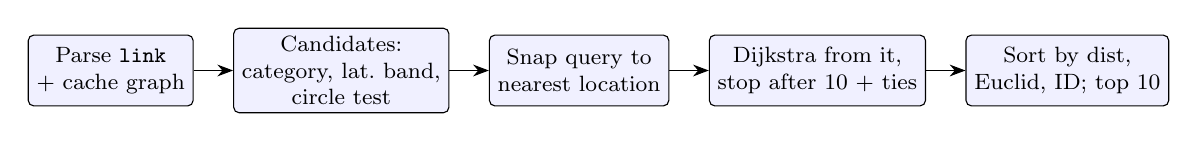
\begin{tikzpicture}[node distance=5mm,
  box/.style={draw,rounded corners=2pt,fill=blue!6,minimum height=9mm,align=center,font=\footnotesize,inner sep=3pt},
  arr/.style={-{Stealth[length=2mm]}}]
  \node[box] (a) {Parse \code{link}\\+ cache graph};
  \node[box,right=of a] (b) {Candidates:\\category, lat.\ band,\\circle test};
  \node[box,right=of b] (c) {Snap query to\\nearest location};
  \node[box,right=of c] (d) {Dijkstra from it,\\stop after 10 + ties};
  \node[box,right=of d] (e) {Sort by dist,\\Euclid, ID; top 10};
  \foreach \x/\y in {a/b,b/c,c/d,d/e} \draw[arr] (\x)--(\y);
\end{tikzpicture}
\caption{Processing of one request.}
\end{figure}

\begin{algorithm}[h]
\caption{\textsc{Search}$(q,\;c,\;r,\;L)$ \quad ($K=10$)}
\begin{algorithmic}[1]
\State $G \gets$ cache lookup by SHA-1 of $L$; if absent, parse $L$ into an undirected, de-duplicated CSR graph (weights per A2)
\State $T \gets \{p : \mathrm{cat}(p)=c,\ \lVert p-q\rVert_2 \le r\}$ \Comment{lat.\ band by binary search, then circle test}
\State $s \gets \arg\min_p \lVert p-q\rVert_2$ \Comment{start node (A3)}
\State $d[s]\gets 0$; push $(0,s)$ on a min-heap; $F\gets[\,]$; $\textit{cut}\gets\infty$
\While{heap not empty}
  \State pop $(d,u)$; \textbf{skip} if $u$ already settled; \textbf{stop} if $d>\textit{cut}$
  \If{$u\in T$}
     \State append $(\mathrm{round}(d),\ \lVert u-q\rVert,\ \mathrm{ID}(u))$ to $F$
     \State \textbf{if} $|F|=K$ \textbf{then} $\textit{cut}\gets d$ \quad\textbf{if} all of $T$ found \textbf{then stop}
  \EndIf
  \ForAll{road $(u,v)$ with length $w$} relax: if $d+w<d[v]$ update and push \EndFor
\EndWhile
\State \Return IDs of the first $K$ entries of $F$ sorted lexicographically
\end{algorithmic}
\end{algorithm}

\subsection{Correctness}
Dijkstra's algorithm with non-negative weights settles vertices in non-decreasing order of true road distance $d(s,\cdot)$.
Hence the first $K$ valid locations popped have the $K$ smallest distances. Continuing until the popped distance is
\emph{strictly} larger than the $K$-th one collects every location tied with the $K$-th, so the final lexicographic sort
(distance, Euclidean distance, ID) is deterministic and independent of heap order. Unreachable locations are never popped and
are therefore never returned. Distances are rounded to $10^{-9}$ only to remove floating-point summation error.

\subsection{Complexity}
Parsing costs $O(|L|\log|L|)$ once per \emph{distinct} file (cached, LRU of three). Candidate selection is $O(\log n+m)$ with $m$
the number of same-category points in the latitude band. Snapping is one $O(n)$ vectorised pass. The search itself is
$O(E'\log V')$ on the explored region $(V',E')$, which in practice is a small ball around $s$; the worst case is $O(E\log V)$.

%------------------------------------------------------------------------------
\section{API Implementation}
Implemented in Python with FastAPI, NumPy and pandas; the CSV is loaded once at start-up.

\begin{table}[h]\centering\small
\begin{tabular}{@{}p{3.6cm}p{11.2cm}@{}}\toprule
\textbf{Item} & \textbf{Behaviour}\\\midrule
Route & \code{/search/} (GET or POST); also accepts \code{/search}\\
Fields & \code{lat}, \code{long}, \code{cat} (case-insensitive), \code{rad}, \code{link}\\
\code{link} accepted as & uploaded file (multipart); file text in a form, JSON or query field; JSON list of \code{[a,b]} pairs; an \code{http(s)} URL; a file name inside the app folder. If omitted: \code{links.txt} if present, else a full lattice (Manhattan fallback)\\
Response & \code{\{"ids": [id1, id2, ..., id10]\}}, nearest first\\
Errors & 422 missing/non-numeric field; 400 unknown category, negative radius, empty or invalid link file\\
Link parsing & tolerant: CRLF, blank and \code{\#} comment lines, commas, duplicate or reversed pairs, self-loops, unknown IDs and junk lines are ignored\\\bottomrule
\end{tabular}
\caption{API contract.}
\end{table}
Example (the file is uploaded with the request):
\begin{lstlisting}
curl -X POST http://HOST/search/ -F lat=0.5 -F long=0.5 -F cat=bank -F rad=0.1 -F link=@links.txt
{"ids":[4850,4948,4947,4648,5349,5348,5449,5347,5155,5452]}
\end{lstlisting}
(The IDs above come from \code{sample\_links.txt}, a network with 15\% of roads removed.) Blocking work runs in a thread pool so
that the server stays responsive.

%------------------------------------------------------------------------------
\section{Experimental Evaluation}
\subsection{Correctness}
Every result is compared with an \emph{independent} implementation (separate parser, SciPy Dijkstra, plain-Python filtering and sorting).
\begin{table}[h]\centering\small
\begin{tabular}{@{}p{10.4cm}r@{}}\toprule
\textbf{Check} & \textbf{Result}\\\midrule
4{,}000 random queries on networks with 0, 5, 15 and 30\% of roads missing (half start on a location, half off-grid) & 0 mismatches\\
Uploads, 15\% missing, both weight modes (60 queries each) & 120/120\\
Seven ways of sending \code{link} (upload, GET+upload, form, JSON text, JSON pairs, URL, file name) & 7/7\\
Messy file (CRLF, comments, commas, duplicates, junk) & 15/15\\
45\% of roads missing (many unreachable nodes) & 30/30\\
Complete road file $=$ no-link Manhattan fallback $=$ Dijkstra & 40/40\\
Errors, case-insensitive category, 10 unique IDs, category and radius constraints & pass\\\bottomrule
\end{tabular}
\caption{Validation; reproduced by \code{python3 test\_api.py}.}
\end{table}


\subsection{Performance}
\begin{table}[h]\centering\small
\begin{tabular}{@{}lrr@{}}\toprule
 & \textbf{10k nodes} & \textbf{1M nodes (synthetic)}\\\midrule
Roads in link file & 16{,}805 & 1{,}897{,}916\\
CSV load + index (start-up, once) & 15\,ms & 1.4\,s\\
Parse + build graph (once per distinct file) & 11\,ms & 4.1\,s\\
Search, median & 0.15\,ms & 4.9\,ms\\
Search, 99th pct.\ / max & 0.43\,ms / 0.56\,ms & -- / 6.7\,ms\\
Peak memory (process) & -- & $\approx$0.96\,GB\\\bottomrule
\end{tabular}
\caption{Latency on one CPU core (\code{python3 bench.py}). 10k: radii 0.1--1.5; 1M: radius 0.05, 5\% roads missing.}
\end{table}
\begin{lstlisting}
$ python3 bench.py
validate: 4000 queries (0/5/15/30% roads missing), mismatches vs scipy Dijkstra: 0
baselines: mean matches of 10 vs the link-aware answer (600 queries per row, radii .15/.25/.4)
  missing | Euclid-only | Manhattan-only
      2%  |        9.34 | 9.94
      5%  |        9.34 | 9.82
     10%  |        9.29 | 9.55
     15%  |        9.21 | 9.31
     30%  |        8.43 | 8.37
timing: 10k nodes, 16805 links: CSV load+index 15 ms, parse+build 11 ms,
        search median 0.15 ms, p99 0.43 ms, max 0.56 ms
ties: coords vs hops, 800 queries with 10 answers: sets differ in 10.8%,
      avg overlap 9.94/10
\end{lstlisting}
Both are far below any practical limit; the 1M-node run shows the method scales beyond the required 10{,}000 locations.

\subsection{What the link file changes}
Figure~\ref{fig:base} measures how many of the true 10 (road-distance) answers are recovered by two baselines that ignore the roads:
Euclidean ranking and Manhattan ranking (the no-link fallback). Each point is the mean of 600 queries.
\begin{figure}[h]\centering
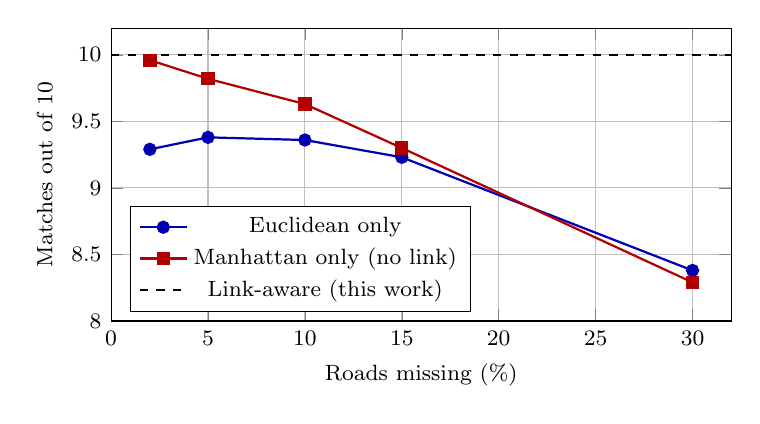
\begin{tikzpicture}
\begin{axis}[width=0.78\linewidth,height=5.3cm,xlabel={Roads missing (\%)},ylabel={Matches out of 10},
 ymin=8,ymax=10.2,xmin=0,xmax=32,legend pos=south west,legend style={font=\footnotesize},
 grid=major,tick label style={font=\footnotesize},label style={font=\footnotesize}]
\addplot[thick,mark=*,blue!70!black] coordinates {(2,9.29)(5,9.38)(10,9.36)(15,9.23)(30,8.38)};
\addplot[thick,mark=square*,red!70!black] coordinates {(2,9.96)(5,9.82)(10,9.63)(15,9.30)(30,8.29)};
\addplot[thick,dashed,black] coordinates {(0,10)(32,10)};
\legend{Euclidean only,Manhattan only (no link),Link-aware (this work)}
\end{axis}
\end{tikzpicture}
\caption{Agreement of road-ignoring baselines with the road-aware answer.}\label{fig:base}
\end{figure}
Manhattan ranking is nearly right when few roads are missing but degrades steadily; at 30\% missing, both baselines lose
about 1.6 of 10 answers per query. Using the link file removes this error, which is what the task rewards.

\subsection{Ties and the edge-weight model}\label{sec:ties}
On a lattice many locations tie exactly. In \code{coords} mode, edge lengths come from the 6-decimal CSV coordinates, so lattice-equal
locations differ by up to $\approx2\cdot10^{-6}$ and that decides ties (then Euclidean distance, then ID); this reproduces a reference
that sums coordinate-based edge lengths. In \code{hops} mode ties are genuine and are broken by Euclidean distance, then ID.
Comparing the two on 800 queries, the top-10 \emph{sets} differ in 10.8\% of them, with an average overlap of 9.94 of 10. The
modes therefore differ only in which of several equally good places is chosen at the cut-off.

%------------------------------------------------------------------------------
\section{Limitations and Design Choices}
\begin{itemize}
\item \textbf{Hidden conventions.} The statement does not specify edge weights, tie-breaking or how an off-grid start is handled. We chose
 the most natural reading (A1--A4) and provide switches; a different convention in the reference changes at most a few boundary answers per query.
\item \textbf{Undirected roads.} If the reference treats links as one-way, results can differ.
\item \textbf{Start node.} The nearest location is used even if it has no roads; then only that location is reachable. The task guarantees
 at least 10 valid locations, which implies a usable start.
\item \textbf{Fewer than 10 reachable.} Fewer IDs are returned rather than inventing unreachable ones.
\item \textbf{Memory.} Building a 1M-node graph peaked at $\approx$0.96\,GB (transient parsing lists plus Python-list CSR); the 10k case is negligible. The LRU keeps at most three graphs, so very large networks would need a smaller cache.
\end{itemize}

%------------------------------------------------------------------------------
\section{Reproducibility and Deployment}
\noindent\begin{minipage}{\linewidth}
\begin{lstlisting}
nearest_api/
  app.py               # API
  locations.csv        # dataset (next to app.py)
  requirements.txt     # dependencies
  test_api.py          # validation suite
  sample_links.txt     # example road file (15% of roads missing)
  REPORT.pdf / .tex    # this report
\end{lstlisting}
\end{minipage}\par\smallskip
\noindent\begin{minipage}{\linewidth}
\begin{lstlisting}
pip install -r requirements.txt
uvicorn app:app --host 0.0.0.0 --port 8000     # run the API
python test_api.py                              # run the tests
\end{lstlisting}
\end{minipage}\par\smallskip
For submission, deploy the folder to a web host with these build and start commands:
\begin{lstlisting}
build:  pip install -r requirements.txt
start:  uvicorn app:app --host 0.0.0.0 --port $PORT
\end{lstlisting}
API link: \code{http://10.1.75.51:6269/search/}\\
GitHub link: \url{https://github.com/harshitap1305/CSD-Proximity-Search-API}

%------------------------------------------------------------------------------
\section{Conclusion}
Treating the problem as a shortest-path query on a request-supplied graph gives an exact answer: candidates are filtered by the
circle, ranked by road distance with an early-stopping Dijkstra search, and ordered deterministically. The implementation matched an
independent reference on every validation query, runs in well under a millisecond on the given data, scales to a million nodes, and
accepts the road file in every reasonable transport format. The residual risk lies in conventions the statement leaves open (edge
weights, ties, start-point handling), which we made explicit and configurable.
\end{document}